\documentclass[12pt, letterpaper]{article}
\usepackage{graphicx} %LaTeX package to import graphics
\graphicspath{{images/}} %configuring the graphicx package

\title{Wikinger shit}
\author{Alli ussered em Philipp\thanks{De Rüeremer no use}}
\date{31.Okotber 2023}
\begin{document}
\maketitle
We have now added a title, author and date to our first document!
Hello, World!
Hello this is a test
\begin{figure}
    \centering
    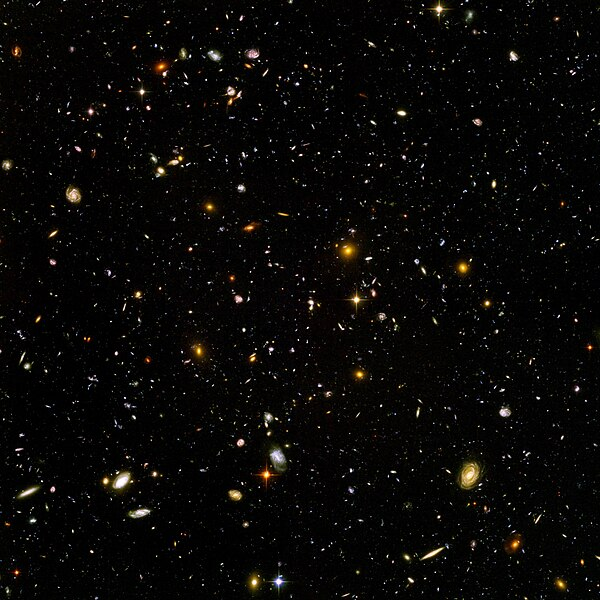
\includegraphics[width=0.75\textwidth]{delte_me_1}
    \caption{A nice plot.}
    \label{fig:delte_me_11}
\end{figure}
hahahah aklsdjflajsdl dfghjhgfddf
Some of the \textbf{greatest and most remarkable}
discoveries in \underline{science} ere made by \textbf{\textit{accident}}.
As you can see in figure \ref{fig:delte_me_11}, the function grows near the origin. This example is on page \pageref{fig:delte_me_11}.
\end{document}